Upon the construction of a complete request, the Client Side Application 
must call a third-party API to process the request. Since there 
is no apriori information regarding the ammount of time necessary to process the request,
the implementation of this crucial step should be asynchronous.
This means that users can continue to interact with the application, while the request is being processed.

The businnes logic of the developed application is managed by Redux, but Redux by itself is not able
to create asynchronous behaviour. In order to do so, it is necessary to use two secondary libraries:
redux-thunk, and superagent. \textit{Redux-thunk} is a store enhancer, or a middleware,
providing additional functionalities to the store,
and \textit{superagent} is a library for asynchronous javascript and XML (AJAX) requests.

While Redux defines that an action must return a pure javascript object, Redux-thunk overwrites this behaviour,
and lets an action return a function instead. Thus, an asynchronous action 
is an action which upon being completed, invokes a function, which dispatches a secondary action.
This means that an asynchronous action may update the state two times: the first when the action is initially dispatched,
and a second time when the request is complete.
In order to inform the user that the request is being processed, the primary action should 
update the state with some waiting information, while the secondary action interacts with the API.

The details of the asynchronous action previously explained are illustrated in figure \ref{fig:ajax_request}.
Note that an asynchronous request starts with an user defined action, dispatched from inside a component,
and updates the Redux store at two particular moments in time: the first immediatly, and the second after receiving the asynchronous response.

\begin{figure}[htpb]
  \centering
  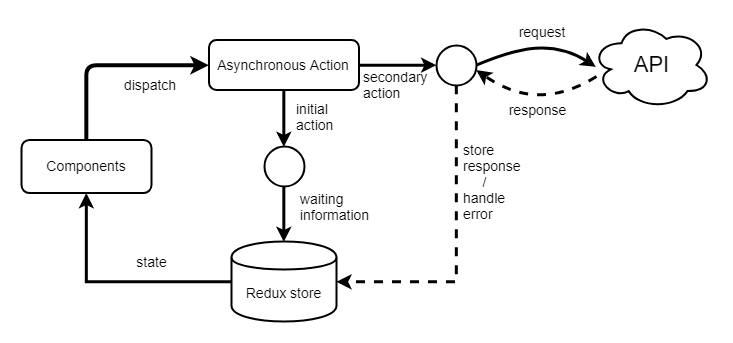
\includegraphics[width=\textwidth]{./Figures/system_implementation/async_request.png}
  \caption{Asynchronous javascript request.}
  \label{fig:ajax_request}  
\end{figure}

The actual request to the third-party API corresponds to a simple HTTP request to a particular URL,
according to the API protocol defined in subsection \ref{sec:api_protocol}. The URL extenstion, called 
the Uniform Resource Identifier (URI), enables the specification of the particular resource under request.
Thus, the URI may be implemented as a way of specifying the attributes which characterize the user selected resource.
It follows thats a particular resource is identified by a collection of (key, value) pairs,
which identify the resource attribute and its user defined value.
There are a total of 7 keys which may be used to construct a request: flyFrom, returnTo, flyTo, startDate, endDate, duration and tripType.
